% =====================================================================
%  OUTLINE PENELITIAN
%  Struktur: judul, ringkasan, state of the art, tema utama,
%            referensi, arsitektur (bagan alur)
%  Hilma Amalia Putri — Informatika, Fakultas Teknik, Universitas Siliwangi
%  Kompilasi: bash build.sh
% =====================================================================

\documentclass[12pt,a4paper,oneside]{report}

\ifdefined\XeTeXversion
  \usepackage{fontspec}
  \IfFileExists{fonts/times.ttf}{
    \setmainfont{times.ttf}[Path=fonts/, BoldFont=timesbd.ttf,
      ItalicFont=timesi.ttf, BoldItalicFont=timesbi.ttf]
  }{\usepackage{mathptmx}}
\else
  \usepackage[T1]{fontenc}\usepackage[utf8]{inputenc}\usepackage{mathptmx}
\fi

\usepackage[english,indonesian]{babel}
\usepackage[a4paper,top=4cm,left=4cm,bottom=3cm,right=3cm]{geometry}
\usepackage{setspace}
\doublespacing
\usepackage{indentfirst}
\setlength{\parindent}{1.27cm}

\usepackage{etoolbox}
\makeatletter
\def\ps@isita{%
  \let\@mkboth\@gobbletwo
  \def\@oddhead{\hfil\normalfont\normalsize\thepage}%
  \def\@evenhead{\normalfont\normalsize\thepage\hfil}%
  \def\@oddfoot{}\def\@evenfoot{}}
\makeatother
\pagestyle{isita}

\usepackage{titlesec}
\renewcommand{\thechapter}{\arabic{chapter}}
\renewcommand{\thesection}{\thechapter.\arabic{section}}
\titleformat{\chapter}[display]{\centering\bfseries\normalsize}
  {\thechapter}{0pt}{\MakeUppercase}
\titlespacing*{\chapter}{0pt}{0pt}{1.5\baselineskip}
\titleformat{\section}{\bfseries\normalsize}{\thesection}{0.6em}{}
\titleformat{\subsection}{\bfseries\normalsize}{\thesubsection}{0.6em}{}

\usepackage{graphicx}
\usepackage{float}
\usepackage{booktabs}
\usepackage{tabularx}
\usepackage{array}
\newcolumntype{L}[1]{>{\raggedright\arraybackslash}p{#1}}
\renewcommand{\tabularxcolumn}[1]{>{\raggedright\arraybackslash}m{#1}}
\usepackage{caption}
\captionsetup{font=small,labelfont=bf,labelsep=period,
  justification=centering,singlelinecheck=false}
\captionsetup[table]{position=top,skip=0.5\baselineskip}
\captionsetup[figure]{position=bottom,skip=0.5\baselineskip}
\AtBeginEnvironment{tabularx}{\singlespacing\small\setlength{\tabcolsep}{4pt}}
\counterwithin{table}{chapter}
\renewcommand{\thetable}{\thechapter.\arabic{table}}
\counterwithin{figure}{chapter}
\renewcommand{\thefigure}{\thechapter.\arabic{figure}}

\usepackage{enumitem}
\newlist{poin}{enumerate}{2}
\setlist[poin]{label=\alph*.,ref=\alph*.,leftmargin=*,align=left,
  itemsep=0pt,topsep=0.25\baselineskip}
\newlist{urut}{enumerate}{2}
\setlist[urut]{label=\arabic*.,ref=\arabic*.,leftmargin=*,align=left,
  itemsep=0pt,topsep=0.25\baselineskip}

\usepackage{tikz}
\usetikzlibrary{arrows.meta,positioning,fit,backgrounds}
\usepackage[round,authoryear]{natbib}
\bibliographystyle{plainnat}
\newcommand{\parencite}[1]{\citep{#1}}
\newcommand{\textcite}[1]{\citet{#1}}
\usepackage[hidelinks]{hyperref}

% =====================================================================
\begin{document}

\begin{titlepage}
  \centering
  \vspace*{0.5cm}
  {\bfseries\normalsize OUTLINE PENELITIAN TUGAS AKHIR\par}
  \vspace{1.2cm}
  {\bfseries\normalsize DEKODING TERBIMBING DAN VERIFIKASI BERLAPIS\\[0.2cm]
   PADA TAMPILAN TUJUH SEGMEN\\[0.2cm] TIMBANGAN DIGITAL\par}
  \vspace{1.2cm}
  {\normalsize Tahap model, menuju sistem pencatatan yang dapat dipakai\par}
  \vspace{2cm}
  {\normalsize Hilma Amalia Putri\\[0.2cm] [NPM]\par}
  \vspace{2cm}
  {\bfseries\normalsize JURUSAN INFORMATIKA\\[0.2cm]
   FAKULTAS TEKNIK UNIVERSITAS SILIWANGI\\[0.2cm] TASIKMALAYA\par}
  \vspace{1cm}
  {\normalsize [Bulan] 2026\par}
\end{titlepage}

\pagenumbering{roman}
\pagestyle{plain}
\tableofcontents
\clearpage
\listoftables
\clearpage
\listoffigures

\clearpage
\pagenumbering{arabic}
\pagestyle{isita}

% =====================================================================
\chapter{Judul}

\section{Judul yang Diajukan}

\begin{quote}
\textbf{Dekoding Terbimbing dan Verifikasi Berlapis pada Tampilan Tujuh
Segmen Timbangan Digital}
\end{quote}

Judul itu memuat metode (dekoding terbimbing dan verifikasi berlapis) dan objek
(tampilan tujuh segmen timbangan digital), dengan panjang sebelas kata. Nama model
tidak dimasukkan karena judul bertahan sampai sidang, sedangkan model berganti
generasi dalam hitungan bulan: PP-OCRv5 terbit 2026 \parencite{zhang2026ppocrv5}
dan PP-OCRv6 menyusul pada tahun yang sama \parencite{zhang2026ppocrv6}.

Tujuan tidak dicantumkan di judul. Kalimat "untuk menekan kesalahan senyap" akan
membawa judul menjadi lima belas kata, melewati batas dua belas kata pada acuan
penulisan judul. Tujuan itu dipindahkan ke bagian ringkasan dan tema utama.

\section{Judul Alternatif}

\begin{poin}
  \item Verifikasi Berlapis dan Dekoding Terbimbing untuk Menekan Kesalahan Senyap
        (sebelas kata, tanpa objek yang spesifik).
  \item Pembacaan Tampilan Tujuh Segmen Timbangan Digital dengan Dekoding
        Terbimbing (sebelas kata, tanpa kata verifikasi).
\end{poin}

% =====================================================================
\chapter{Ringkasan dan Gambaran Umum}

\section{Masalah di Lapangan}

Timbangan digital di gudang menampilkan berat pada panel tujuh segmen. Angka itu
dibaca operator, lalu ditulis ke buku atau dimasukkan ke aplikasi. Pekerjaan
tersebut berulang puluhan sampai ratusan kali per hari, dan kesalahan ketik tidak
terlihat setelah tercatat. Pada tampilan yang sama, ``1006,5'' dan ``106,5'' hanya
berbeda satu digit nol; keduanya terbaca wajar di kertas.

Kamera ponsel dapat memotret panel itu dan sebuah model pengenalan karakter dapat
membacanya. Persoalannya bukan apakah model bisa menghasilkan angka. Persoalannya
adalah menentukan apakah angka yang dihasilkan layak dipercaya, pada saat angka itu
dihasilkan, ketika berat sebenarnya belum diketahui siapa pun.

\section{Apa yang Sudah Dicapai Penelitian}

Pembacaan tampilan tujuh segmen sudah dikerjakan sejak 2019 dengan angka yang
tinggi. Pendekatan klasik non-pembelajaran mesin melaporkan 99,7\% pada 1.146
karakter dengan waktu 20 milidetik pada timbangan elektronik
\parencite{jiang2026method}. CRNN-CTC dengan pra-pemrosesan YOLO melaporkan
\textit{exact match} 90,37\% (197 dari 218 citra) dan CER 3,6\% pada data logger
tujuh segmen \parencite{effendi2025unjuk}. YOLO dengan kepala inferensi digit
mencapai 97,8\% per bingkai pada 30 bingkai per detik \parencite{yenneti2023lightweight},
sedangkan generator citra sintetis dengan model digit dan model titik desimal
terpisah mencapai 96,8\% untuk perangkat berspesifikasi rendah
\parencite{gushima2023automatic}.

Laporan itu menunjukkan dua hal sekaligus. Model sudah cukup baik untuk membaca
panel yang terlihat jelas, dan setiap laporan berhenti pada satu bilangan, yaitu
akurasi pada kumpulan data penulisnya sendiri.

\section{Apa yang Ditawarkan Penelitian Ini}

Penelitian ini bekerja pada dua tempat di dalam alur yang sama.

Yang pertama berada di dalam model, pada tahap penguraian keluaran menjadi teks.
Dekoder CTC mengasumsikan batas antar karakter tidak diketahui, sehingga dua digit
kembar hanya dapat dihasilkan bila ada satu langkah kosong di antaranya
\parencite{graves2006ctc}. Pada panel tujuh segmen, batas itu justru terlihat:
jumlah slot, lebar tiap slot, dan posisi titik desimal dapat dihitung dari profil
proyeksi citra. Penelitian ini memakai informasi tersebut untuk membatasi
penguraian, lalu mengukur akibatnya pada digit kembar dan titik desimal.

Yang kedua berada di luar model, pada tahap memutuskan. Keluaran model diperiksa
oleh empat lapis aturan yang tidak bergantung pada piksel: jumlah digit terhadap
jumlah slot, kewajaran berat untuk suatu produk, kesepakatan antar bingkai, dan
nilai keyakinan yang telah dikalibrasi. Hasil akhirnya bukan string, melainkan
keputusan terima, tolak, atau minta konfirmasi, beserta alasan yang menyertainya.

\section{Arah Akhir}

Tujuan akhir penelitian adalah sistem pencatatan timbangan yang dipakai operator,
bukan model yang berhenti di meja eksperimen. Sistem itu membaca panel dari kamera
ponsel, menampilkan angka yang diterima, menolak angka yang meragukan dan meminta
timbang ulang, lalu menyimpan citra beserta keputusan dan alasannya sebagai jejak
audit. Karena gudang sering berada di lokasi dengan jaringan lemah, model berjalan
di perangkat tanpa koneksi. Penelitian ini mengerjakan bagian yang menentukannya,
yaitu model dan lapisan keputusan; antarmuka, basis data, dan pengujian oleh
operator dikerjakan setelah bagian itu terbukti.

% =====================================================================
\chapter{State of the Art}

\section{Lima Kelompok Pendekatan}

Literatur yang dipakai penelitian ini dapat dipetakan menjadi lima kelompok
(Tabel~\ref{tab:kelompok}).

\begin{table}[H]
\caption{Pemetaan pendekatan pembacaan tampilan tujuh segmen}
\label{tab:kelompok}
\begin{tabularx}{\textwidth}{@{}L{2.9cm} L{4.1cm} L{3.9cm} X@{}}
\toprule
\textbf{Kelompok} & \textbf{Sumber} & \textbf{Hasil yang dilaporkan} & \textbf{Keterbatasan} \\
\midrule
Klasik non-pembelajaran mesin & \textcite{jiang2026method}; \textcite{auerswal_ssocr} & 99,7\% pada 1.146 karakter, 20 milidetik & Bergantung kondisi citra; perilaku saat gagal tidak dilaporkan \\
Deep learning khusus tujuh segmen & \textcite{effendi2025unjuk}; \textcite{gushima2023automatic}; \textcite{yenneti2023lightweight}; \textcite{bonilla2023adapting}; \textcite{oicws2026lcd}; \textcite{low2024detecting} & 90,37\% \textit{exact match}; 96,8\%; 97,8\% per bingkai; 98\% pada 800 citra & Seluruhnya berhenti pada akurasi kumpulan data sendiri \\
Kumpulan data dan tolok ukur & \textcite{laroca2019convolutional}; \textcite{kanagarathinam2019text} & 2.000 citra dan 10.000 anotasi tingkat digit; citra mentah meter energi & Mayoritas objeknya meter energi, bukan timbangan \\
Pengenalan karakter umum generasi baru & \textcite{zhang2026ppocrv6}; \textcite{zhang2026ppocrv5} & 83,2\% rata-rata 15 kategori pada 34,5 juta parameter & Mengklaim menangani tampilan digital, diuji pada tujuh segmen belum \\
Model bahasa-visi & \textcite{ega2026leveraging}; \textcite{lin2026measurebench} & \textit{Full-string recognition} 93,85\%; terbaik 30,2\% pada data nyata & Akurat pada transkripsi, lemah pada inferensi skala; butuh jaringan \\
\bottomrule
\end{tabularx}
\end{table}

\section{Dua Angka yang Tampak Bertentangan}

\textcite{ega2026leveraging} melaporkan \textit{full-string recognition} 93,85\%
untuk Gemini pada perangkat ukur digital. Pada tahun yang sama, MeasureBench
melaporkan model bahasa-visi terbaik hanya mencapai 30,2\% pada 2.442 citra nyata
yang mencakup 26 jenis alat ukur \parencite{lin2026measurebench}.

Keduanya tidak saling membantah. Pengujian pertama menilai transkripsi digit yang
telah tersusun pada panel, sedangkan pengujian kedua menuntut pembacaan skala dan
penalaran spasial. Bagi penelitian ini, yang penting adalah akibatnya: model
bahasa-visi unggul pada transkripsi tetapi tidak dapat diandalkan untuk memutuskan
benar atau salahnya bacaan, dan biayanya tidak sebanding dengan model 34,5 juta
parameter yang berjalan luring.

\section{Mengapa Akurasi Tidak Menjawab Persoalan}

Akurasi dihitung setelah nilai sebenarnya diketahui. Pada eksperimen, nilai itu ada
karena peneliti membandingkan keluaran model dengan label. Di gudang, nilai itu
justru yang sedang dicari, sehingga akurasi tidak tersedia saat keputusan harus
diambil.

Akurasi juga tidak menyebut bacaan mana yang salah. Dua sistem dengan akurasi sama
dapat berbeda sepuluh kali pada jumlah kesalahan yang lolos tanpa peringatan
(Tabel~\ref{tab:dua-sistem}).

\begin{table}[H]
\caption{Dua sistem dengan akurasi identik dan keandalan berbeda}
\label{tab:dua-sistem}
\begin{tabularx}{\textwidth}{@{}L{6.4cm} L{3.2cm} L{3.2cm}@{}}
\toprule
\textbf{Ukuran} & \textbf{Sistem A} & \textbf{Sistem B} \\
\midrule
Akurasi pada data uji & 90\% & 90\% \\
Bacaan salah yang ditandai meragukan & 0 dari 10 & 9 dari 10 \\
Kesalahan senyap & 10\% & 1\% \\
\bottomrule
\end{tabularx}
\end{table}

Sistem A lebih berbahaya karena angka besarnya membuat operator berhenti memeriksa.
Pada 90\% akurasi, satu dari sepuluh catatan masuk tanpa diketahui, dan pada
ratusan transaksi per hari itu berarti puluhan catatan keliru per minggu.

\section{Celah Penelitian}

Lima celah berikut disusun dari literatur di atas. Setiap celah disertai bagian
penelitian ini yang menutupnya.

\begin{table}[H]
\caption{Celah penelitian dan bagian yang menutupnya}
\label{tab:celah}
\begin{tabularx}{\textwidth}{@{}L{0.9cm} L{5.4cm} L{4.2cm} X@{}}
\toprule
\textbf{Kode} & \textbf{Celah} & \textbf{Bukti celah} & \textbf{Ditutup oleh} \\
\midrule
G1 & Tidak ada laporan terukur tentang bacaan mana yang gagal, hanya rata-rata akurasi & Semua laporan pada Tabel~\ref{tab:kelompok} berhenti pada satu bilangan & Kandidat 1, lewat laju kesalahan senyap per kategori \\
G2 & Geometri slot diketahui tetapi tidak dipakai membatasi penguraian CTC & \textcite{oicws2026lcd} mencatat kegagalan CTC pada digit kembar tanpa menyelesaikannya & Kandidat 2, lewat dekoding terbimbing \\
G3 & Titik desimal diperlakukan sebagai masalah terpisah, bukan bagian dari penguraian & \textcite{gushima2023automatic} memakai model desimal tersendiri & Kandidat 2, lewat batasan posisi pada tiap slot \\
G4 & Belum ada luaran berupa keputusan layak atau tidak layak & Seluruh sistem mengembalikan string & Kandidat 1, lewat keputusan tiga nilai \\
G5 & Belum ada pengukuran \textit{risk--coverage} pada domain ini & Metrik yang dipakai selalu FSR dan CER & Kandidat 1, lewat AURC dan \textit{selective accuracy} \\
\bottomrule
\end{tabularx}
\end{table}

\section{Pernyataan Celah Penelitian}

Dari Tabel~\ref{tab:celah}, celah yang dapat dituntaskan penelitian ini adalah
ketiadaan hubungan terukur antara keluaran model dan kelayakan keluaran itu.
Literatur membaca panel tujuh segmen sebagai tugas pengenalan karakter: masuk citra,
keluar string, dinilai dengan akurasi. Akibatnya dua pertanyaan yang menentukan
pemakaian di lapangan tidak pernah dijawab. Pertama, kesalahan seperti apa yang
tersisa dan berapa banyak yang lolos tanpa peringatan. Kedua, apakah informasi
geometri panel yang sudah terlihat di citra dapat dipakai untuk menekan kesalahan
itu sebelum sampai ke operator.

Penelitian ini menjawab keduanya dengan mengukur, bukan dengan menambah model
baru: kesalahan digit kembar dan titik desimal diukur sebelum dan sesudah dekoding
terbimbing, dan kesalahan senyap diukur sebelum dan sesudah verifikasi berlapis.
Kedua pengukuran memakai data uji yang sama sehingga hasilnya dapat dibandingkan
satu sama lain dan dengan angka pada Tabel~\ref{tab:kelompok}.

% =====================================================================
\chapter{Tema Utama}

\section{Model Dasar: PP-OCRv6}

PP-OCRv6 dirilis 2026 dalam tiga tingkat berukuran 1,5 juta, 7,7 juta, dan 34,5
juta parameter \parencite{zhang2026ppocrv6}. Laporan itu menyebut tampilan digital
sebagai salah satu sasaran, dan pada 15 kategori pengujian, tingkat menengah
mencapai 83,2\% rata-rata berbobot, naik 5,1 poin dari PP-OCRv5 \textit{server}.
Angka itu dilaporkan penulisnya \parencite{zhang2026ppocrv6} dan belum diuji
pada tampilan tujuh segmen oleh pihak lain, sehingga penelitian ini tidak boleh
menganggapnya berlaku.

Susunan modelnya berlapis. Tulang punggung pengenal memakai PPLCNetV4, dilanjutkan
pengode \textit{EncoderWithLightSVTR} yang mengubah peta ciri menjadi urutan
vektor. Kepala keluarannya dua: CTC dan NRTR. Pada saat inferensi hanya kepala CTC
yang dipakai \parencite{zhang2026ppocrv6}. Jumlah parameter kepala pengenal tingkat
\textit{small} sekitar 5,2 juta dan tingkat \textit{medium} sekitar 19 juta
\parencite{zhang2026ppocrv6}, sedangkan PP-OCRv5 sebesar 5 juta
\parencite{zhang2026ppocrv5}.

Pilihan model ini punya dua akibat yang harus dinyatakan di depan. Pertama, karena
kepala yang dipakai adalah CTC, perilaku keluaran mengikuti sifat CTC, termasuk
masalah digit kembar yang dijelaskan pada Bagian~4.3. Kedua, karena ukurannya kecil,
model dapat berjalan di perangkat tanpa koneksi, yang menjadi syarat arah akhir
penelitian.

\section{Kandidat 1: Verifikasi Kontekstual}

\subsection{Gagasan}

Model mengembalikan string. Verifikasi mengubah string itu menjadi keputusan
dengan menambahkan pemeriksaan yang tidak berasal dari piksel. Pemeriksaan itu
memakai pengetahuan tentang alat, produk, dan waktu penimbangan, bukan tentang
tampilan.

\subsection{Empat Lapis}

\begin{poin}
  \item Lapis struktural. Jumlah karakter pada keluaran dibandingkan dengan jumlah
        slot hasil profil proyeksi. Bacaan lima digit dari panel enam slot ditolak.
        Posisi titik desimal juga diperiksa: titik hanya boleh berada di antara
        slot, dan hanya satu.
  \item Lapis fisik. Berat dibandingkan dengan rentang sah produk yang dipilih
        operator. Karung 25 kilogram yang terbaca ``2,5'' ditolak, begitu pula
        bacaan di luar toleransi timbangan.
  \item Lapis temporal. Tiga sampai lima bingkai diambil berurutan. Bacaan yang
        seluruhnya sama diterima; bacaan yang berubah pada satu digit ditandai
        untuk konfirmasi. Jarak antar bacaan dipakai sebagai ukuran kesepakatan.
  \item Lapis statistik. Nilai keyakinan model dikalibrasi pada kumpulan data
        kalibrasi yang terpisah dari data uji, lalu dipakai sebagai ambang.
        Kalibrasi penting karena nilai keyakinan mentah CTC cenderung terlalu
        tinggi pada bacaan salah.
\end{poin}

\subsection{Keluaran dan Ukurannya}

Keluaran setiap bacaan berupa salah satu dari tiga nilai: terima, tolak, atau
konfirmasi, dengan alasan berupa lapis mana yang memutuskan. Tiga ukuran yang
dilaporkan mengikuti cara kerja itu. \textit{Coverage} adalah persentase bacaan
yang diterima otomatis. \textit{Selective accuracy} adalah akurasi pada bacaan yang
diterima. Laju kesalahan senyap adalah persentase bacaan salah yang diterima tanpa
peringatan, dan angka inilah yang menjadi ukuran utama karena ia yang paling mahal
akibatnya.

\section{Kandidat 2: Dekoding Terbimbing Geometri}

\subsection{Mengapa Penguraian Menjadi Persoalan}

CTC memberi keluaran berupa distribusi peluang pada setiap langkah waktu, dengan
satu kelas tambahan berupa \textit{blank}, lalu menggabungkan langkah yang sama dan
membuang \textit{blank} \parencite{graves2006ctc}. Karena batas antar karakter
tidak diketahui model, dua karakter yang sama berurutan hanya dapat muncul bila ada
\textit{blank} di antaranya. Ketika dua digit kembar berdempetan dan tampak serupa,
langkah kosong itu tidak terbentuk, dan model menghasilkan satu digit alih-alih
dua. Pada panel tujuh segmen, pola inilah yang mengubah ``1006,5'' menjadi
``106,5''; kegagalan sejenis tercatat pada implementasi YOLO dan CRNN untuk layar
tujuh segmen \parencite{oicws2026lcd}.

Titik desimal punya masalah sendiri. Tingginya tiga sampai lima piksel, jauh lebih
kecil dari digit, dan pada ukuran tertentu ia tidak memperoleh langkah waktu
tersendiri. Salah satu penelitian menyiasatinya dengan melatih model titik desimal
terpisah dari model digit \parencite{gushima2023automatic}, yang berarti strukturnya
ditambahkan di luar penguraian, bukan di dalamnya.

\subsection{Geometri yang Sudah Terlihat}

Pada tampilan tujuh segmen, tata letak tidak acak. Digit berdiri pada garis dasar
yang sama dengan lebar yang hampir seragam, dipisahkan jarak tetap, dan titik
desimal berada tepat di garis dasar. Profil proyeksi vertikal citra menunjukkan
keenam hal itu sebagai lembah dan puncak: setiap slot menjadi satu kelompok kolom
berisi, dan setiap pemisah menjadi lembah mendekati nol.

Dari situ diperoleh tiga hal yang dapat dipakai pengurai: jumlah slot N, batas kiri
dan kanan setiap slot, serta posisi calon titik desimal. Informasi itu diketahui
sebelum model bekerja dan tidak bergantung pada bobot model.

\subsection{Usulan}

Dekoding terbimbing menambahkan batasan ke dalam pencarian berkas, bukan mengubah
bobot model terlebih dahulu.

\begin{poin}
  \item Berkas mencatat slot yang sudah terisi. Satu slot hanya boleh
        menghasilkan satu emisi karakter; emisi kedua pada slot yang sama diberi
        penalti, bukan langsung dibuang, agar keputusan tetap dapat ditelusuri.
  \item \textit{Blank} wajib disisipkan di antara dua slot bertetangga yang
        karakternya sama, karena tanpa itu penggabungan CTC akan menghapus salah
        satunya.
  \item Titik desimal hanya boleh muncul pada posisi calon yang ditemukan profil
        proyeksi, dan paling banyak satu kali.
  \item Skor setiap hipotesis ditambah suku penalti pelanggaran geometri, dengan
        bobot yang ditentukan pada data kalibrasi, bukan pada data uji.
\end{poin}

Pembandingnya tiga dekoder pada model yang sama: \textit{greedy}, berkas tanpa
batasan, dan berkas dengan batasan. Selisih ketiganya menunjukkan sumbangan
batasan geometri secara terpisah dari sumbangan pencarian berkas.

\subsection{Varian Pelatihan}

Batasan di atas bekerja saat inferensi tanpa melatih ulang. Varian kedua
menambahkan penalti saat pelatihan: label yang membuat satu slot menghasilkan lebih
dari satu karakter diberi penalti pada fungsi kerugian, sehingga model belajar
menghasilkan \textit{blank} di tempat yang benar. Kedua varian dibandingkan karena
yang pertama murah dan yang kedua berpotensi lebih baik tetapi menuntut pelatihan
ulang.

\section{Kedua Kandidat dalam Satu Alur}

Kandidat 2 bekerja sebelum keluaran ada, kandidat 1 bekerja sesudahnya. Urutannya
tidak dapat dibalik: verifikasi memeriksa jumlah digit terhadap jumlah slot, dan
pemeriksaan itu baru bermakna bila penguraian tidak lagi menghapus digit kembar.
Sebaliknya, dekoding terbimbing tidak dapat memutuskan apakah bacaan layak dipakai,
karena ia tidak mengetahui berat produk maupun riwayat penimbangan.

Karena itu keduanya diukur berurutan pada satu kumpulan data uji: model dasar,
model dasar dengan dekoding terbimbing, lalu dekoding terbimbing dengan verifikasi
berlapis. Setiap tahap dilaporkan dengan metrik yang sama.

\section{Tujuan Akhir: Sistem yang Dipakai}

Bagian ini menjelaskan bentuk akhir yang dituju, agar arah pekerjaan tahap model
tidak kehilangan sasarannya.

\begin{poin}
  \item Alur kerja. Operator memilih produk, memotret panel, dan menerima satu dari
        tiga keadaan: angka diterima dan tercatat, angka ditolak dengan alasan, atau
        angka diminta dikonfirmasi. Pada keadaan ketiga, operator menimbang ulang
        atau memasukkan angka secara manual.
  \item Berjalan luring. Model 34,5 juta parameter dijalankan di perangkat.
        Koneksi hanya dipakai untuk menyinkronkan catatan yang sudah tersimpan,
        bukan untuk membaca panel \parencite{zhang2026ppocrv6}.
  \item Jejak audit. Setiap transaksi menyimpan citra, string mentah, keputusan,
        dan lapis yang memutuskan. Tanpa itu, kesalahan tidak dapat ditelusuri
        setelah terjadi.
  \item Ukuran penerimaan. Selain metrik model, sistem dinilai dari tingkat
        koreksi operator, waktu per transaksi, dan jumlah timbang ulang yang
        dipicu. Ketiganya diukur pada pengujian terbatas di satu lokasi.
\end{poin}

\section{Cara Mengukur}

\begin{table}[H]
\caption{Rancangan pengukuran}
\label{tab:ukur}
\begin{tabularx}{\textwidth}{@{}L{1.0cm} L{5.2cm} L{4.4cm} X@{}}
\toprule
\textbf{Kode} & \textbf{Konfigurasi} & \textbf{Ukuran} & \textbf{Pertanyaan} \\
\midrule
E1 & Model dasar, dekoder \textit{greedy} & FSR, CER, akurasi desimal & Sejauh mana kemampuan dasar? \\
E2 & Model dasar, dekoder berkas & FSR, latensi & Apakah pencarian berkas cukup? \\
E3 & Berkas dengan batasan geometri & FSR, error digit kembar, akurasi desimal & Berapa sumbangan geometri? \\
E4 & Batasan ditambah penalti latihan & FSR, latensi, biaya latih & Apakah pelatihan ulang sepadan? \\
E5 & Tanpa verifikasi & Laju kesalahan senyap & Berapa kesalahan yang lolos? \\
E6 & Verifikasi lapis 1 sampai 3 & Laju kesalahan senyap, \textit{coverage} & Lapis mana yang menangkap paling banyak? \\
E7 & Ditambah lapis 4 terkalibrasi & \textit{Coverage}, \textit{selective accuracy}, AURC & Di mana titik seimbangnya? \\
\bottomrule
\end{tabularx}
\end{table}

Seluruh eksperimen memakai satu kumpulan data uji yang dikunci sebelum E1 berjalan.
Data latih dibangkitkan secara sintetis dengan kondisi terkontrol, sedangkan data
uji memuat citra timbangan nyata, karena data uji sintetis hanya akan mengukur
ketidaksempurnaan pembangkitnya sendiri \parencite{gushima2023automatic}. Model
pembanding di luar PP-OCRv6, yaitu CRNN-CTC \parencite{shi2017crnn}, DBNet dengan
PARSeq \parencite{low2024detecting, bautista2022parseq}, dan ssocr
\parencite{auerswal_ssocr}, dijalankan pada data uji yang sama sebagai batas bawah
dan batas atas.

% =====================================================================
\chapter{Referensi}

Dua puluh empat sumber dipakai pada outline ini. Tabel~\ref{tab:sumber} memetakan kode sumber ke sitasi singkatnya, dan daftar lengkap beserta DOI ada pada Bibliografi di bagian akhir.

\begin{table}[H]
\caption{Sumber yang dipakai dan kodenya}
\label{tab:sumber}
\begin{tabularx}{\textwidth}{@{}L{1.1cm} L{4.5cm} L{1.2cm} X@{}}
\toprule
\textbf{Kode} & \textbf{Sitasi} & \textbf{Tahun} & \textbf{Venue} \\
\midrule
S01 & Effendi, dkk. & 2025 & JIIF 9(2) 107--115 \\
S02 & Ega, dkk. & 2026 & BEEI 15(5) 4239--4252 \\
S03 & Laroca, dkk. & 2019 & J. Electron. Imaging 28(1) 013023 \\
S04 & Low, dkk. & 2024 & ITM Web of Conferences 63 01007 \\
S05 & Kulkarni, dkk. & 2021 & Frontiers in Artificial Intelligence 4 543176 \\
S06 & Xiang, dkk. & 2026 & Sensors 26(1) 265 \\
S07 & Gushima dan Kashima & 2023 & PHM Society Asia-Pacific Conference \\
S08 & Yenneti, dkk. & 2023 & Electronic Imaging 35(7) 282 \\
S09 & Jiang dan Li & 2026 & Proc. SPIE \\
S10 & Fu, dkk. & 2026 & Journal of Imaging 12(4) 146 \\
S11 & Wei, dkk. & 2023 & Algorithms 16(4) 192 \\
S12 & Kanagarathinam dan Sekar & 2019 & Energy Reports 5 842--852 \\
S13 & Lin, dkk. & 2026 & CVPR 2026 (arXiv:2510.26865) \\
S14 & Zhang, dkk. (a) & 2026 & arXiv:2606.13108 \\
S15 & Valente, dkk. & 2025 & arXiv:2508.21732 \\
S16 & Bonilla-Rivas, dkk. & 2023 & ICCNS 19--25 \\
S17 & OICWS & 2026 & GitHub: lcd-digit-recognition \\
S18 & Auerswal & t.t. & ssocr, perangkat lunak \\
S19 & Shi, dkk. & 2017 & IEEE TPAMI 39(11) \\
S20 & Graves, dkk. & 2006 & ICML \\
S21 & Sheng, dkk. & 2019 & ICDAR \\
S22 & Zhang, dkk. (b) & 2026 & arXiv:2603.24373 \\
S23 & Charles, dkk. & 2021 & WACV \\
S24 & Bautista dan Atienza & 2022 & ECCV (arXiv:2207.06966) \\
\bottomrule
\end{tabularx}
\end{table}

\chapter{Arsitektur dan Bagan Alur}

\section{Bagan Alur}

Alur penelitian berjalan satu arah dari citra sampai keputusan. Kandidat 2 berada
di dalam kotak model, pada tahap penguraian; kandidat 1 berada sesudahnya, pada
tahap keputusan. Kotak bergaris putus-putus di bawah menandai bagian yang menjadi
tujuan akhir dan belum dikerjakan pada tahap ini.

\begin{figure}[H]
\centering
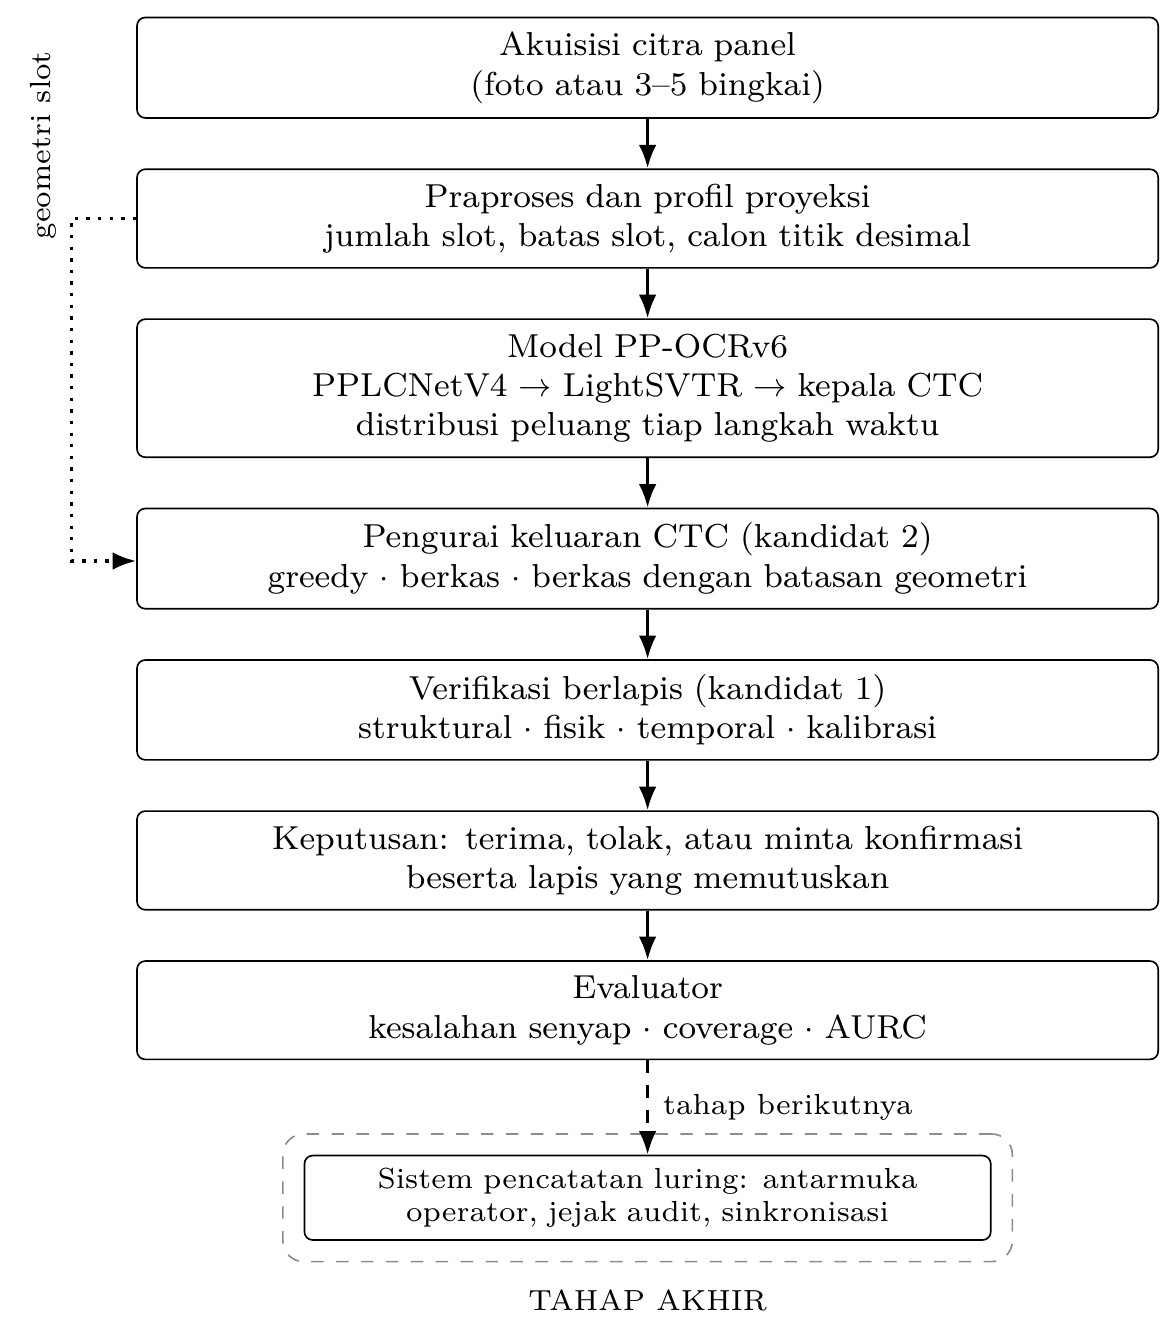
\includegraphics[width=0.95\textwidth,height=13.6cm,keepaspectratio]{gambar/alur-model.png}
\caption{Arsitektur penelitian: dekoding terbimbing di dalam model, verifikasi berlapis sesudahnya}
\label{fig:alur-model}
\end{figure}

\section{Penjelasan Blok}

\begin{table}[H]
\caption{Blok arsitektur, masukan, dan keluaran}
\label{tab:blok}
\begin{tabularx}{\textwidth}{@{}L{3.1cm} L{3.4cm} L{3.4cm} X@{}}
\toprule
\textbf{Blok} & \textbf{Masukan} & \textbf{Keluaran} & \textbf{Alasan} \\
\midrule
Akuisisi & Foto atau 3--5 bingkai & Citra dan metadata & Lapis temporal memerlukan beberapa bingkai \\
Praproses & Citra penuh & Area panel, profil proyeksi & Profil dipakai dua kali: memotong panel dan menghitung slot \\
Model PP-OCRv6 & Area panel & Peta ciri dan distribusi tiap langkah waktu & Tulang punggung PPLCNetV4 dengan pengode LightSVTR \\
Pengurai & Distribusi langkah waktu & String dan skor & Titik kerja kandidat 2 \\
Verifikasi berlapis & String dan konteks & Keputusan beralasan & Titik kerja kandidat 1 \\
Evaluator & Keputusan dan label & Kesalahan senyap, coverage, AURC & Ukuran keandalan, bukan akurasi \\
Sistem pencatatan & Keputusan & Catatan, citra, jejak audit & Tujuan akhir, dikerjakan setelah lapisan model \\
\bottomrule
\end{tabularx}
\end{table}

\section{Urutan Kerja}

\begin{urut}
  \item Menyiapkan data: pembangkit sintetis untuk latih, pengambilan citra nyata
        untuk uji, lalu mengunci data uji.
  \item Menjalankan model dasar tanpa perubahan dan mencatat angka E1 sebagai
        titik awal.
  \item Membangun ekstraksi slot dari profil proyeksi dan mengujinya pada 50 citra
        sebelum dipakai.
  \item Menerapkan dekoding terbimbing, menjalankan E3, lalu E4 bila hasil E3
        menunjukkan perbaikan yang berarti.
  \item Menambahkan lapis verifikasi satu per satu dan mengukur penurunan
        kesalahan senyap pada setiap penambahan.
  \item Menyusun kurva \textit{risk--coverage} dari E7 sebagai hasil utama.
  \item Mengulang seluruh pengukuran dengan CRNN-CTC, DBNet-PARSeq, dan ssocr
        sebagai pembanding.
\end{urut}

\section{Batas Tahap Ini}

Antarmuka, basis data, sinkronisasi, dan pengujian oleh operator tidak dikerjakan
pada tahap ini. Ketiganya bertumpu pada satu asumsi, yaitu lapisan model dan
verifikasi sudah terbukti menurunkan kesalahan senyap. Membangun antarmuka lebih
dahulu akan menghasilkan aplikasi yang rapi dengan mesin yang belum terukur.

\clearpage
\bibliography{references}

\end{document}
